\input chapter_jps2/table_expansion

\section{Comparison with JPS 2011}
\label{sec::results}

We first analyse the impact on JPS search performance for various combinations
of our optimisation techniques: JPS (B), which adds block-based jumping, JPS
(B + P) which combines block-based jumping with improved pruning, JPS+ which
adds pre-processing and JPS+ (P) which combines pre-processing with improved
pruning.  To avoid confusion we will denote the original algorithm as JPS
2011.

\begin{sidewaysfigure*}[p] 
\begin{center}
		   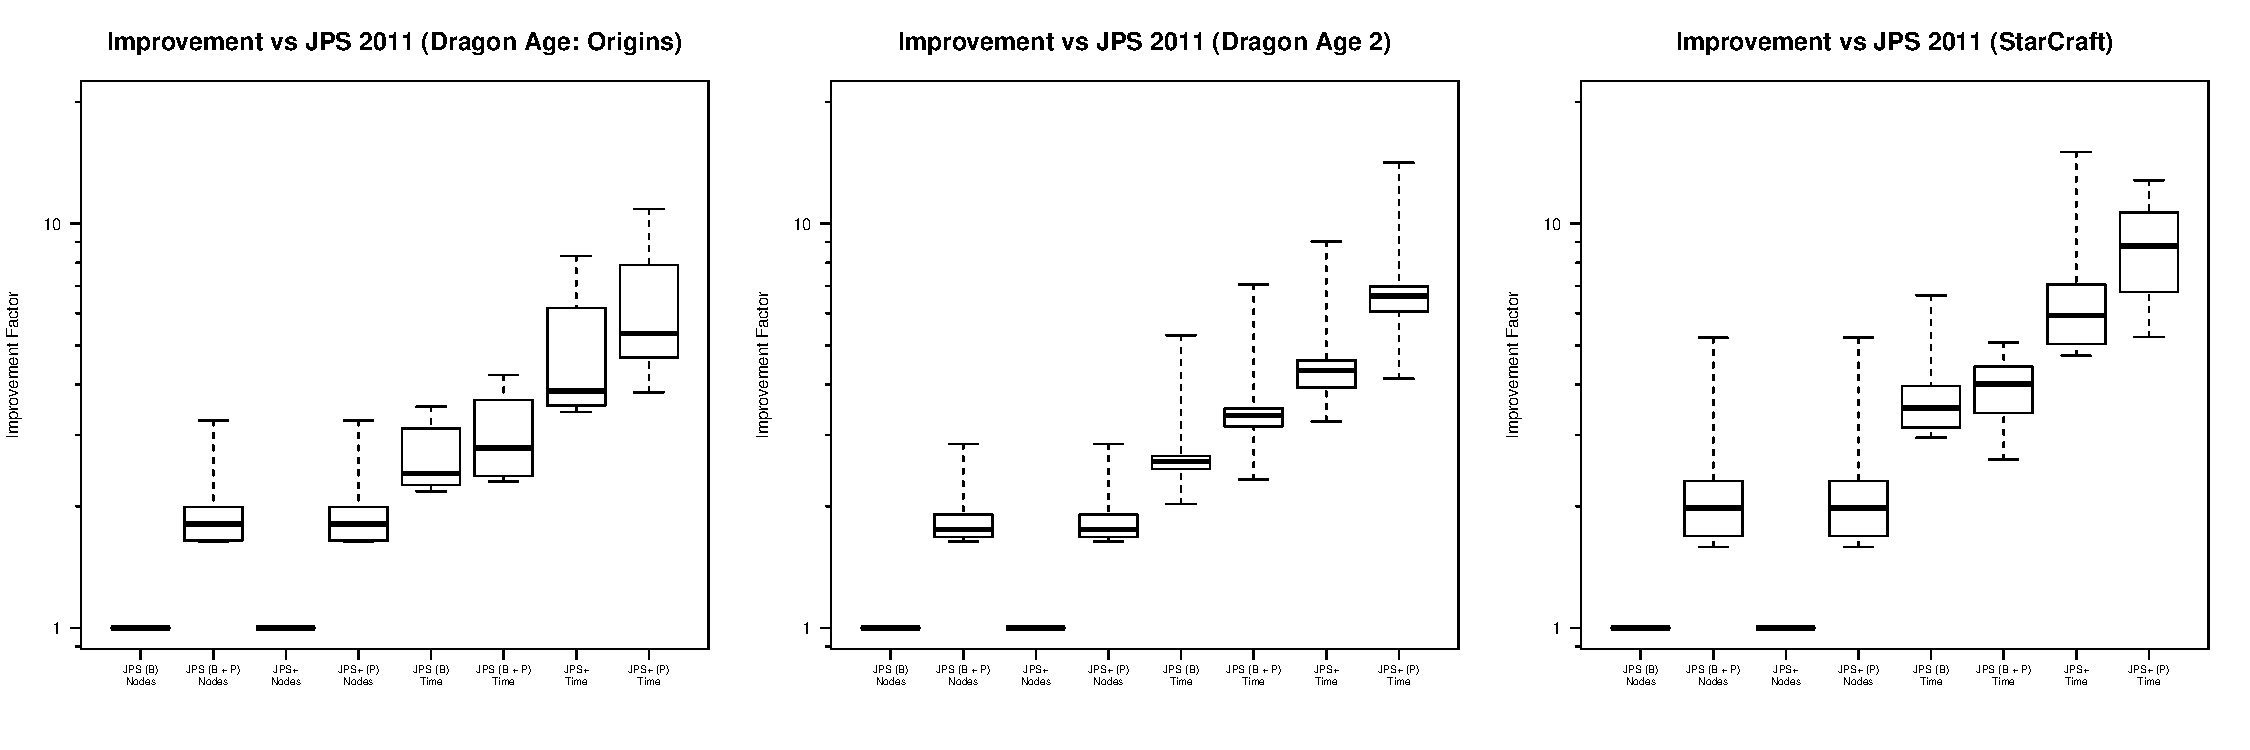
\includegraphics[width=\columnwidth, trim = 0mm 0mm 0mm 0mm]
			{chapter_jps2/diagrams/improvement_vs_jps.pdf}
       \end{center}
\caption[Performance of improved JPS variants vs. original JPS] 
{\small We measure the relative performance (or improvement factor) of each of
our new JPS variants against the original. We consider two metrics: nodes
expanded and search time. An improvement factor of 2 for search time means
twice as fast; for node expansions it means half as many nodes expanded.
Higher values are always better. 
Each boxplot shows the distribution of results.
We give five figures; from
bottom to top in each case: min, 1st quartile, median, 3rd quartile and max.
}
\label{fig::jps2::vs_jps2011}
\end{sidewaysfigure*}

We have previously observed that the bottleneck of the JPS 2011 algorithm is
individual node expansion operations. In Table~\ref{table::jps2::expansion} we
give results for the average time required to expand (i.e. generate all
successors of) one million random starting nodes from each input map in each
benchmark set. We find that block-based jumping and pre-processing jump points
each improve average times by one and two orders of magnitude respectively vs.
JPS 2011.  Pruning intermediate jump points from the search tree increases the
average branching factor by several times but the time-per-expansion is still
much better.  In Figure~\ref{fig::jps2::vs_jps2011} we give a summary of
search performance, in terms of time and node expansions, for all GPPC
instances on each of our three benchmark sets.  In each case and for each
metric we consider relative improvement vs. JPS 2011.  We show the spread of
results after having assigned all test instances into buckets of similar
cost.  We observe that any of our alternative approaches is strictly faster
than the original.  Moreover, JPS (B) and JPS (B + P) have all the same
advantages as JPS 2011: they are fast, optimal, online and require, in
principle at least, no extra memory vs. JPS 2011 (recall that in practice we
store a rotated copy of map twice to improve memory access patterns).  A
summary of pre-processing requirements is given in
Table~\ref{table::jps2::preproc}. Note that JPS+ and JPS+ (P) have the same
requirements and are not listed separately.

\input chapter_jps2/table_preproc

\section{Comparison with SUB}
SUB~\cite{urasKH13} is a recent pathfinding technique from the literature.
As one of the joint winners of the 2012 Grid-based Path Planning Competition (GPPC) 
SUB has been shown to be very fast and is considered the current state of the art.
We compare against two variants described by the original authors: SUB-S (S
for Simple) and SUB-TL (TL for Two Level). The former is guaranteed optimal
while the latter is not.  To evaluate SUB-S and SUB-TL we used the authors'
original C++ implementation which we obtained from~{\small
\url{http://gppc-2012.googlecode.com/svn/trunk/entries/SUB-a/}}.

%The basic version of the algorithm, which its authors term SUB-S (S for Simple),
%is both complete and optimal. 
%This algorithm works by pre-computing a grid analogue of a
%visibility graph, called a subgoal graph, which it stores and searches instead of the original grid. 
% An improved variant termed SUB-TL (TL for Two Level)
%further prunes the pre-processed graph by directly connecting pairs of nodes for
%which the local heuristic is perfect (this operation is similar to graph contraction~\cite{geisberger08}
%in that it has the effect of pruning any intermediate nodes along the way).
%To avoid a large growth in its branching-factor SUB-TL also prunes other additional 
%edges from the graph but this latter step makes the algorithm sub-optimal in certain cases.

Table~\ref{table::jps2::preproc} compares the pre-processing requirements of 
SUB-S and SUB-TL with JPS+ (JPS+ (P) has identical requirements and is not shown). 
We observe that both JPS+ and SUB are able to pre-process most maps in well under a second 
and in most cases using less than 10MB of memory. A small number of notable exceptions 
arise for both JPS+ and SUB-TL.
%Notable exceptions include one StarCraft map on which SUB-TL needed more than 23 seconds of 
%pre-processing time and one DA:O map for which JPS+ required over 21MB of space 
%(c.f. 0.2 seconds pre-proc time for JPS+ and $\sim$10MB of space for SUB-TL, respectively).
In Figure~\ref{fig::jps2::vs_sub} we compare our four JPS variants with SUB-S and SUB-TL across all
game map instances from the 2012 GPPC. We find that JPS (B) and JPS (B + P) are both
competitive with, and often faster than, than SUB-S. Meanwhile, JPS+ (P) appears competitive 
with SUB-TL for a large set of instances.
Across our three benchmarks, DA:O, DA2 and SC, we measured an improvement for 
JPS (B + P) vs. SUB-S in 92\%, 84\% and 89\% of tested instances respectively.
For JPS+ (P) vs. SUB-TL we measured an improvement in 43\%, 77\% and 68\% of 
tested instances respectively.

\begin{sidewaysfigure*}[p] 
\begin{center}
		   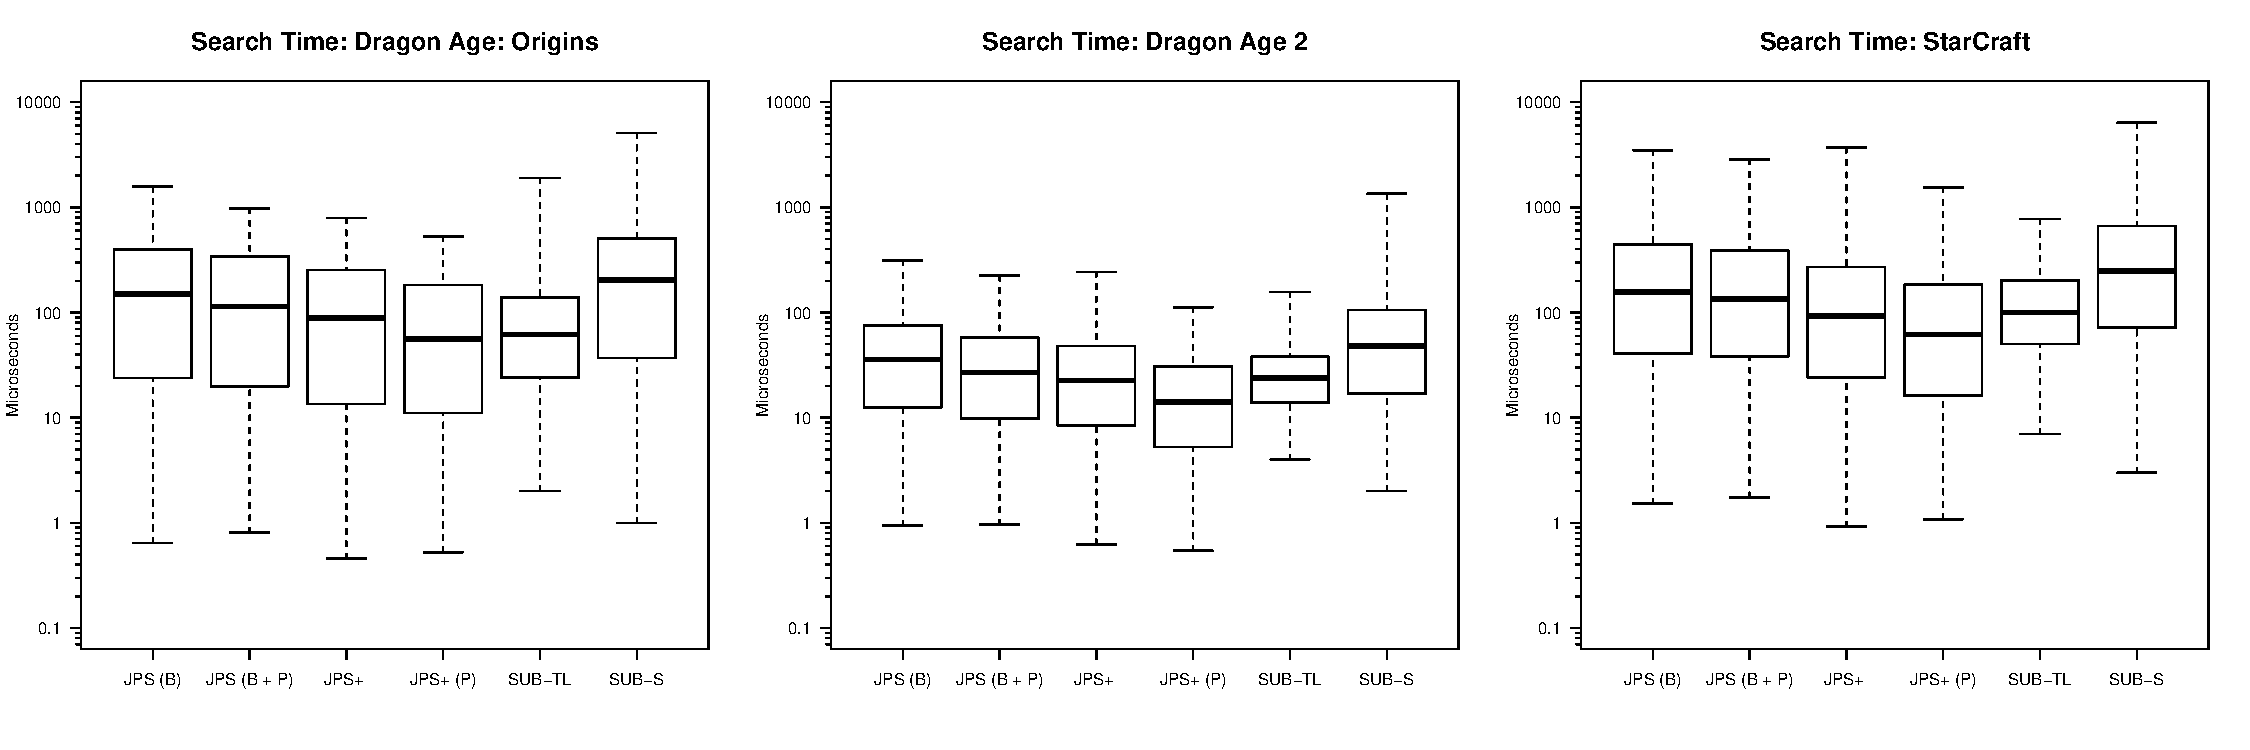
\includegraphics[width=\columnwidth, trim = 0mm 0mm 0mm 0mm]
			{chapter_jps2/diagrams/jps_vs_sub_boxplot.pdf}
       \end{center}
\caption[Search time performance: JPS+ vs. SUB] 
{\small
We compare the raw search time performance of our improved JPS variants (both
online and offline) with two recent and very performant algorithms: simple
subgoal graphs (SUB-S) and two-level subgoal graphs with local edge pruning
(SUB-TL). All JPS variants and SUB-S are provably optimal. SUB-TL is not.
Each boxplot shows the distribution of results.  We give five figures; from
bottom to top in each case: min, 1st quartile, median, 3rd quartile and max.
}
\label{fig::jps2::vs_sub}
\end{sidewaysfigure*}

\section{Analysis}
The results demonstrate the superiority of the approaches presented in this
chapter. In JPS (B) and JPS (B + P) we have improved the performance of
JPS 2011 by several factors all while retaining
the same advantages inherent to the original algorithm: completeness, 
optimality and little-to-no memory overhead. Such results are remarkable as
JPS 2011 has itself been shown to improve the performance of classical
search algorithms such as A* by up to one order of magnitude and more.

We have shown with JPS+ and JPS+ (P) that further improvements are also possible. 
In our experiments we employ an offline pre-processing step together with a small 
amount of memory (10MB or less in most cases) in order to identify apriori all jump 
point successors of each grid node.
The main advantage is performance: JPS+ and JPS+ (P) can improve the search times of 
JPS 2011 by up to one order of magnitude and more.
The main disadvantage is that if the map changes the pre-processed
database needs to be re-computed. We have shown that each such pre-computation
can be performed very fast -- usually on the order of tens or hundreds of 
milliseconds. Moreover the pre-computation can be easily parallelised over
several time slices with JPS (B + P) employed as a fallback algorithm in
the interim.

We have compared our JPS-based approaches against two variants of SUB: a very fast 
and very recent preprocessing-based pathfinding technique which was judged to be 
among the most performant entrants in the 2012 Grid Based Path Planning Competition. 
The first variant, SUB-S guarantees optimality; the second, SUB-TL, does not. 
We find that across most benchmark instances JPS (B) and 
JPS (B + P) are not only competitive with but faster than SUB-S. When we compare
JPS+ (P) and SUB-TL we find the two algorithms often have complementary strengths:
JPS+ (P) always has low pre-processing requirements, always finds the optimal path
and is faster on a majority class of tested instances; SUB-TL has low space
requirements and quickly finds optimal or near-optimal solutions to a large class 
of remaining instances.

%JPS (B)'s improvement is over one order of magnitude to the point
%where the additional pruning rule provides only another $10\%$ improvement.
%JPS+ (P) gives another order of magnitude; this demonstrates that a
%substantial amount of time of JPS is spent in finding the next jump point and
%that any improvement in this direction is beneficial.
%
%The bottom part of Figure~\ref{fig::speedup} shows a nice correlation 
%between the total runtime and the number of nodes expanded.  
%Clearly the JPS family's performance 
%can be explained by how it quickly identifies 
%nodes that can be skipped.  
%
%%Next, we turn our attention to Figure~\ref{fig::expansion_time} which measures
%performance in terms of the average time, in mico-seconds, needed to expand a single node.
%It is interesting to observe that in each case the lowest values are attributed to A*. 
%JPS (B) and JPS (B+P), which both perform online symmetry breaking, always record
%the highest values. These figures are in stark contrast with Figure~\ref{fig::speedup} where
%the opposite is true. These results indicate that although eliminating path symmetries can have
%a dramatic positive effect on overall search time, individual node expansions can incur a 
%significant overhead. Thus, if the start and goal are very close, it is sometimes possible that
%A* will be faster than Jump Point Search. The same is also true if JPS must explore very large
%empty areas which contain nodes that appear promising but e.g. eventually lead to a dead-end.
%
%Figure~\ref{fig::expansion_time} also provides 
%interesting insights for improvement: 
%the on-line version of JPS spends substantial time expanding a single node; 
%any improvement on this side would result 
%in huge performance boost.  
%This includes pre-processing techniques lighter 
%than JPS+.  
%
%
% EOF
